% !TEX root = ../ba_scrreprt_master.tex
% @author Marcel Ruland (2018)

\chapter{Applying \fpmupper}
\label{ch:mining}
\chapterintro{chapter description goes here}

\section{Method}
\label{sec:miningmethod}
The following subsections begin by introducing the raw data \emph{as-is} and then proceed by describing the process of annotating and evaluating the data, thus going steadily from the most concrete to more and more abstract representations. I begin by describing the contents of the video corpus and eventually end with abstract rules\footnote{For the definition of \emph{rule} here, see subsection \ref{ssec:miningmethodapproach}.}.

\subsection{The Nature of the Data}
\label{ssec:miningmethodnature}
The corpus is a collection of 10 mother--infant dyads. Mother and infant were recorded at their own homes during a diaper routine. This routine was chosen because it a)~is an activity known to both mother and infant, b)~is an activity where mother and infant are in direct communication with each other for a relatively long period of time, c)~both mother and infant are free in their expressions. The infant especially is free to make use of body movements and gestures and is not reliant on support from the mother, as might be the case if the infant were sitting. The diaper routine was recorded by two video cameras from two different perspectives, such that all relevant events were clearly visible. Figure \ref{fig:rawvid} gives an impression of this raw data. For a more detailed description of the setup see \citet[\snum{2.1}]{nomikou17} and \citet[\pnum{115~f.}]{nomikou11}.\footnote{But note that while the same setup was used, the inclusion or exclusion of groups or individual subjects in the corpus was different due to the different aims of the studies.} The videos had a mean length of 395~s (\emph{\textsc{sd}}~=~186~s).

\begin{figure}[h]
	\centering
	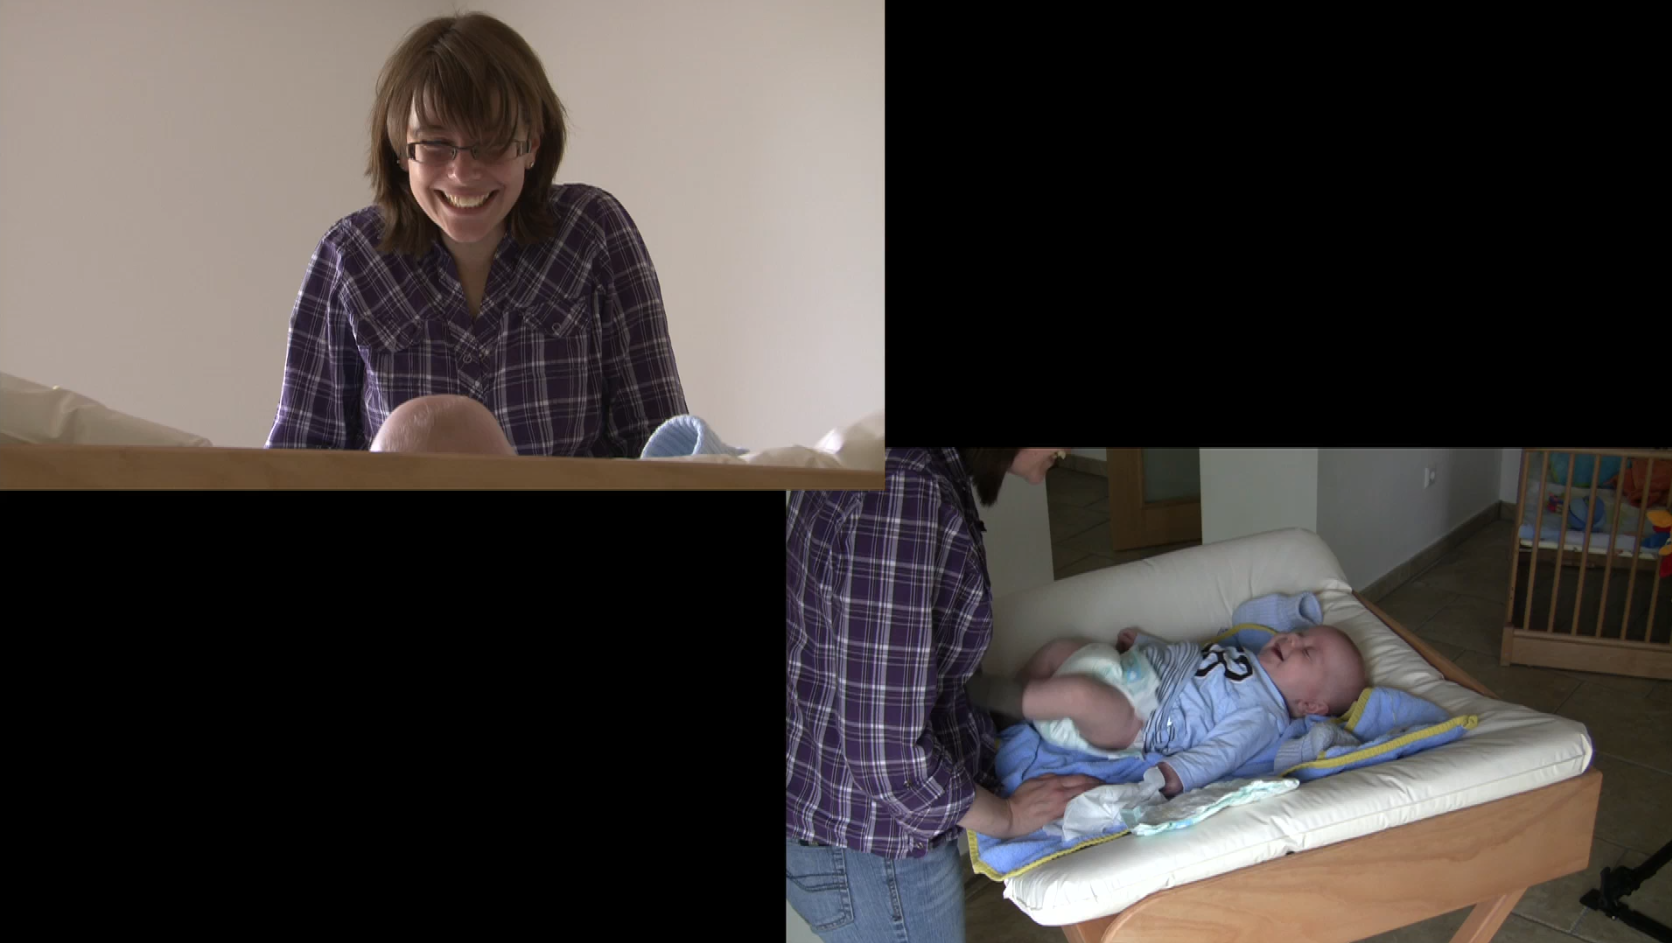
\includegraphics[width=\imgwidth]{../aux/img/video_vp_08_raw.png}
	\label{fig:rawvid}
	\caption{Screen capture of the raw video data}
\end{figure}

\subsection{Annotation of the Videos}
\label{ssec:miningmethodannotation}
11 kinds of events were hand-coded for both mother and child using the \textsc{elan} software \citep{wittenburg06}. These events were of linguistic, vocal, and visual modality. %Categories were chosen HOW??  % ELABORATE here
Table \ref{tab:events} lists all categories. Every annotation contains a start and end time point and therefore also the duration of the respective event. This way, sequences as shown in Figure \ref{fig:idealseq} are obtained (note that this is a fictional sequence). \fpmlabel{A}, \fpmlabel{B}, and \fpmlabel{C} are three different kinds of events; the x-axis represents time. We see two occurrences of type \fpmlabel{A} and \fpmlabel{B} each, as well as a longer occurrence of type \fpmlabel{C}. Those time points that are indicated on the x-axis mark the beginning and/or end time point of a specific occurrence.
\paragraph{A note on terminology}
%A mother--infant pair is referred to as a \emph{dyad.}
One individual occurrence of an event is simply referred to as an \emph{event.}
A specific kind of event is referred to as a \emph{dimension} (i.e.~the data are 11-dimensional, as there are 11 kinds of events).
All events obtained from annotating the recording of a single mother--infant dyad are referred to as a \emph{sequence.}
Finally, all 10 sequences together are referred to as the \emph{corpus.}


\begin{table}[h]
	\centering
	\begin{tabularx}{\textwidth}{>{\ttfamily}lX} 
		\toprule
		{\rmfamily Event}		& Explanation \\
		\cmidrule(lr){1-1} \cmidrule(lr){2-2}
		mother\_speech			& mother speaks \\
		mother\_vocal			& mother vocalises, but does not use language \\
		mother\_gaze\_infant	& mother gazes at infant \\
		mother\_gaze\_object	& mother gazing at object, usually diaper but may be any object \\
		mother\_gaze\_away		& mother gazes neither at infant nor at object \\
		mother\_smile			& mother smiles \\
		\cmidrule(lr){1-1} \cmidrule(lr){2-2}
		infant\_vocal \\
		infant\_gaze\_mother \\
		i\_gaze\_object			& ~ \hfill \textit{analogous to mother's events} \hfill ~ \\
		i\_gaze\_away \\
		infant\_smile \\
		\bottomrule
	\end{tabularx}
	\caption{Events coded in the data}
	\label{tab:events}
\end{table}

\begin{figure}
	\centering
	% !TEX root = ../ba_master.tex
% @author Marcel Ruland (2018)
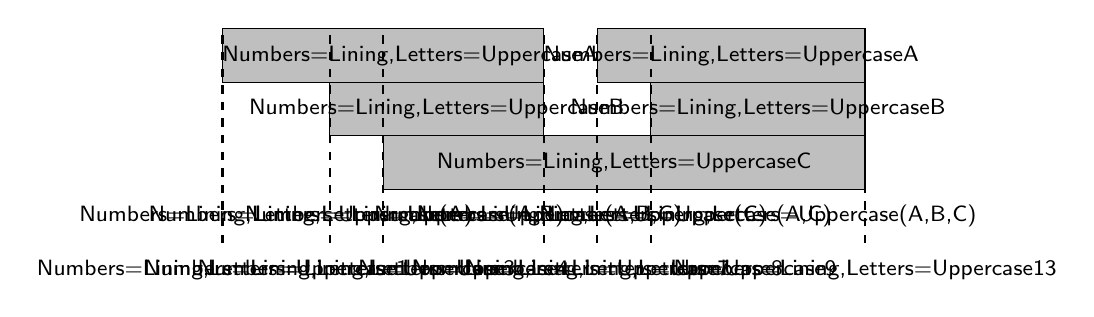
\begin{tikzpicture}[
	scale=0.68,
	every node/.append style={font=\footnotesize\sffamily\addfontfeature{Numbers=Lining,Letters=Uppercase}}]
	% boxes
	\draw [fill=lightgray] (0,4) rectangle (6,5);  % A1
	\node at (3.5,4.5) {A};
	
	\draw [fill=lightgray] (7,4) rectangle (12,5);  % A2
	\node at (9.5,4.5) {A};
	
	\draw [fill=lightgray] (2,3) rectangle (6,4);  % B1
	\node at (4,3.5) {B};
	
	\draw [fill=lightgray] (8,3) rectangle (12,4);  % B2
	\node at (10,3.5) {B};
	
	\draw [fill=lightgray] (3,2) rectangle (12,3);  % C
	\node at (7.5,2.5) {C};
	
	% item sets
	\node at (1,1.5) {(A)};
	\node at (2.5,1.5) {(A,B)};
	\node at (4.5,1.5) {(A,B,C)};
	\node at (6.5,1.5) {(C)};
	\node at (7.5,1.5) {(A,C)};
	\node at (10,1.5) {(A,B,C)};
	
	% time points
	\node at (0,0.5) {1};
	\node at (2,0.5) {3};
	\node at (3,0.5) {4};
	\node at (6,0.5) {7};
	\node at (7,0.5) {8};
	\node at (8,0.5) {9};
	\node at (12,0.5) {13};
	
	% time point lines
	\draw [dashed, thick] (0,1) -- (0,5);
	\draw [dashed, thick] (2,1) -- (2,5);
	\draw [dashed, thick] (3,1) -- (3,5);
	\draw [dashed, thick] (6,1) -- (6,5);
	\draw [dashed, thick] (7,1) -- (7,5);
	\draw [dashed, thick] (8,1) -- (8,5);
	\draw [dashed, thick] (12,1) -- (12,5);
	
	% text representation
%	\node at (6,0) {\code{<(A [1,3]),(A,B [3,4]),(A,B,C [4,7]),(C [7,9])(A,B,C [9,13])>}};
\end{tikzpicture}
	\caption{Graphical representation of an idealised sequence}
	\label{fig:idealseq}
\end{figure}

% wrong position, just for testing
%\begin{figure}
%	\centering
%	% !TEX root = ../../scrreprt/ba_scrreprt_master.tex
% @author Marcel Ruland (2018)
\begin{tikzpicture}
	[every node/.append style={font=\sffamily\addfontfeature{Numbers=Lining}},
	node distance=1cm and 3cm,
	rounded corners,
	align=center,
	>=stealth']
	
	% nodes
	\node [draw] (sig) {\citeauthor{rohlfing18} + \\ significance};
	\node [draw, right=of sig] (reacsig) {\textsc{rt}-data + \\ significance};
	\node [draw, below=of sig] (origin) {\citeauthor{rohlfing18}};
	\node [draw, below=of reacsig] (reac) {\textsc{rt}-data};
	
	% arrows
	\draw [->] (origin) -- node[above] {\footnotesize consider reaction times} (reac);
	\draw [->] (origin) -- node[left]  {\footnotesize establish significance}  (sig);
	\draw [->] (reac)   -- node[right] {\footnotesize establish significance}  (reacsig);
	
	% discussion
%	\node [above right=of reacsig.north west] (discuss) {\footnotesize\textit{3.~extensive discussion}};
	\node at (7.5,1.61) (discuss) {\footnotesize\textit{3.~extensive discussion}};
	\draw[<->, double] (sig.north) to[bend left] node[above]{\footnotesize\textit{2.~comparison}} (reacsig.north);
	\draw[<->, double] (origin.south) to[bend right] node[below]{\footnotesize\textit{1.~comparison}} (reac.south);
	\draw[->, double] (discuss) to (reacsig.north east);
\end{tikzpicture}

















































%	\caption{Method}
%	\label{fig:method}
%\end{figure}

\subsection{Mining Approach}
\label{ssec:miningmethodapproach}
The fundamental aim of \fpmlower\ techniques is to find patterns in a data set that occur \emph{frequently}. The specific kind of pattern and the definition of \emph{frequent} cannot be generalised and depend heavily on the individual application. In contrast to descriptive and inferential statistics, which disprove or affirm hypotheses generated beforehand, \fpmlower\ is of an exploratory, hypothesis-generating nature. Depending on the patterns found, one may then formulate hypotheses afterwards, which may then in turn be tested empirically using descriptive and inferential statistics \cite[\pnum{6~ff.,~tba}]{rohlfing18,han12}.%% ISSUE: How do you give page references for each individual source when citing multiple sources?

\paragraph{Association Rules}
The patterns \citet{rohlfing18} looked for were association rules of the form \fpmrule{A}{B}, where the probability of the succedent \fpmset{B} was high given the antecedent \fpmset{A}. Note that antecedent and succedent are not single events but sets of events. One may equally well form a hypothetical rule of the form \fpmrule{B,D}{A,C,D}. Occurrences of a rule were taken into account if they fulfilled one of two conditions:

\begin{enumerate}
	\item The antecedent's start time point lies before that of the succedent.
	\item The antecedent's and succedent's start time points are identical, i.e.\ they begin at the same time.
\end{enumerate}

Referring again to Figure \ref{fig:idealseq}, one can for example observe the rules \fpmrule{A}{B} and \fpmrule{A}{B, C} (because the start time point of the antecedent lies before that of the succedent), but not \fpmrule{B}{A}.

This scheme can be further adapted to the specific nature of the data. Given that the data are hand-coded and that time points are stored with a precision up tp 1~ms, the second condition will in all probability never be true. Regarding the first condition, the natural imprecision of coding by hand can lead to one annotation beginning before or after another essentially by pure chance, when in fact the two events begin at the same time. The notion of \emph{at the same time} itself is problematic as well. Humans exhibit a certain reaction time to stimuli, which is always greater than 0~ms. It logically follows that if both mother and infant begin exhibiting a certain event \emph{at the same time,} then one event cannot be a reaction to the other because such a reaction would demand an appropriate reaction time. Therefore, an interpersonal rule where both events begin at the same time is the result of pure chance. Not only will it be a meaningless rule, but also an incorrect rule and\dash accordingly\dash should not be captured as a rule at all.

\paragraph{Choosing appropriate delays}  % Clarify this entire paragraph, content is good but confusingly written. Also have a look at the huge ass turn-taking reader for more literature on \rt\ in communication/interaction
Human reaction time (henceforth \rt) correlates with a vast variety of factors, among which are intensity, modality, and complexity of the stimulus \citep{brebner80}, age and gender \citep{der06}, state of alertness \citep{appelle74}, handedness \citep{dane03}, and even personality traits \citep{stelmack93}. Quite obviously, many of those traits cannot be determined for the subjects in the corpus used in the present thesis. However, those factors which are most relevant (namely age of the subject and modality of the stimulus) are both captured in the data and relatively easy to account for. Regarding modality, variation is so small that it may safely be neglected. \citet[\pnum{9}]{brebner80} ascribe the variation to ``differences in the peripheral mechanisms rather than in the central processes'' and give average\footnote{I use the term \emph{average} wherever sources do not state whether the value in question is a mean, median, mode, or other measure of centrality.} \rt s of 8--10~ms for acoustic stimuli and 20--40~ms for visual stimuli to reach the central processes. The resulting difference of 10--32~ms is on a scale so small that considering it would unnecessarily complicate the analysis without providing adequate advantages. Regarding age, mean \rt\ lies  between 1002--1124~ms for infants of age 6--9 months (N~=~24) and between 311--326~ms for adults of age 19--26 years (N=11) \citep[\pnum{95}]{leibold02}.%
\footnote{Stimulus was a pure (i.e.~sine wave) tone of 1000~Hz with loudness ranging from 40--60~dB. No numerical values given. Converted from line chart using the Engauge Digitizer software \citep{mitchell02}. The loudness corresponds to average loudness perceived in conversation \citep[\pnum{32}]{goerne06}} 
Mean infant age in the corpus used for the present thesis is 3~months, mean age of the mothers is XX years. While the infants looked at here are younger than those looked at by \citet{leibold02}, the important point made is that there \emph{is} a difference in reaction time between infants and mothers that must be taken into account. In my analysis, I therefore capture rules of the sort \fpmtextrule{infant}{mother} (i.e.~mother has to react) iff the delay between the start time point of the antecedent is greater than 289~ms before that of the succedent. Similarly, rules of the sort \fpmtextrule{mother}{infant} (i.e.~infant has to react) are captured iff the delay between the start time point of the antecedent is greater than 850~ms before that of the succedent. The values are higher than those given by \citet{leibold02} to account for variation between subjects. The extent of the variation also follows the results of \citet{leibold02}.

I am well aware, that the literature cited with regards to the delays chosen is concerned with \rt\ to generic stimuli and does not consider communication or interaction. Unfortunately, literature specifically concerned with \rt\ in interaction is virtually inexistent. There are some indications that it may be faster than general \rt\ \citep{levinson16}, but none that it may be slower. Therefore, by choosing delays 2 \sd\ below the mean, 95~\% of the actual \rt s will be slow enough to be captured.\footnote{Assuming the distribution to be normally distributed \citep[\pnum{57}]{moore16}} 

For intrapersonal rules only, simultaneous start time points of two events are meaningful. In order to capture them, a further adjustment must be made related to coders' imprecision. The data were annotated frame by frame. Given a rate of 25~fpm, the duration of a single frame is 40~ms. Intrapersonal events with a maximum delay of 40~ms are therefore considered to begin simultaneously. The analysis is formalised in appendix \ref{ch:formalisation}.

% wrong position, just for testing
\begin{figure}
	\centering
	% !TEX root = ../../scrreprt/ba_scrreprt_master.tex
% @author Marcel Ruland (2018)
\begin{tikzpicture}[
		every node/.append style={
			font=\sffamily\addfontfeature{Numbers=Lining}
		},
		node distance=2cm and 2cm
	]
%	\draw[help lines, dashed] (0,0) grid (11,4);
	
	% arrows
	\draw[vecArrow] (0,3) to node {\scriptsize\texttt{speech}} (2,3);
	\draw[vecArrow] (2.5,2) to node {\scriptsize\texttt{speech}} (4.5,2);
	\draw[vecArrow] (6.5,3) to node {\scriptsize\texttt{multimodal}} (10.5,3);
	\draw[vecArrow] (7,2) to node {\scriptsize\texttt{multimodal}} (11,2);
	
	% gaps
	\draw[stealth-stealth] (2,1) to node[above] {\tiny gap} (2.5,1);
	\draw[stealth-stealth] (6.5,1) to node[above] {\tiny gap} (7,1);
	
	% dashed lines
	\draw[dashed] (2,0.5) to (2,4);
	\draw[dashed] (2.5,0.5) to (2.5,4);
	\draw[dashed] (6.5,0.5) to (6.5,4);
	\draw[dashed] (7,0.5) to (7,4);
	
	% annotations
	\node at (2.5,4.5) {\citet{levinson16}};
	\node at (8.5,4.5) {present thesis};
	\node at (-0.5,3) {\texttt{A}};
	\node at (-0.5,2) {\texttt{B}};
\end{tikzpicture}
	\caption{Levinson}
	\label{fig:levinson}
\end{figure}

\section{Results}
\label{sec:miningresults}



































%\subsection{Association Rules}
%In the following, I will first lay out the type of association rule used by \citet{rohlfing18} and then explain how I modified this scheme to better fit the interactional, multimodal nature of the data. The basic sequence is structured as follows:
%\begin{quote}
%	\code{<(A [1,3]),(A,B [3,4]),(A,B,C [4,7]),(C [7,8]),(A,C [8,9]),(A,B,C [9,13])>}
%\end{quote}
%
%In traditional sequential pattern mining, the basic data type---called a sequence---is an ordered set of (unordered) item sets \citep[\pnum{588~ff.}]{han12}. Here, every item set in the sequence has an additional annotation marking the start and end time points between which the item set (that is, one specific occurrence of it) is contained in the data. Figure \ref{fig:idealseq} gives a graphical representation of this example sequence. Rules of the sort \fpmrule{A}{B} must fulfil one of two conditions:
%\begin{enumerate}
%	\item The antecedent's start time point lies before that of the succedent.
%	\item The antecedent's and succedent's start time points are identical, i.e.\ they begin simultaneously.
%\end{enumerate}
%Therefore, in the example sequence one can observe the rules \fpmrule{A}{A,B} but not \fpmrule{B}{A,B}. The following three modifications improve the scheme to better fit the data:
%
%\paragraph{Imprecision of hand-coded data}
%The second condition is problematic given the nature of the data. Every annotation has been hand-coded and with coding by hand comes imprecision. Given the fact that the time points' are precise up to one millisecond, there will in all likelihood not be any two annotations that begin at the exact same point. After examination of the source files (i.e.\ \textsc{elan} files) and consultation with the coders I have decided to allow for a \imprecisiondelay\ delay such that two annotations \(a\) and \(b\) are treated as beginning simultaneously iff their start time points \(s_a\) and \(s_b\) lie no further than 300ms apart (\(|s_a - s_b| < 300ms\)). This delay accounts for the coders' imprecision.
%
%\paragraph{Inter- and intrapersonal rules}
%Given the dyadic nature of the data it is necessary to distinguish between inter- and intrapersonal rules not only in rule evaluation but already in the mining process. Depending on various factors, the average human reaction time to an event lies between XXX and XXXms. %values? source?
%It follows that if both mother and child begin an event at the same time or with a delay below reaction time, then the cooccurrence is pure chance and should not be considered a pattern. Analogous to the maximum delay described in the previous paragraph, interpersonal sequences are only considered with a minimum delay of \reactiontime\ between the time start points.